\subsection{Filastruder-sensor diámetro-bobinadora}
\label{sec:FSB}

Como primera aproximación e intentando asemejar el esquema de producción que tienen en la fábrica de Huesca se va a seguir el siguiente esquema:

	\begin{figure}[H]
            \centering
            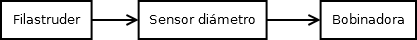
\includegraphics[width=0.6\textwidth]{images/producciones/Diagram1.png}
            \caption{Esquema de producción}
            \label{fig:esquemap_FSB}
    \end{figure}

A la hora de hacer pasar el polímero a través de la boquilla




La boquilla de la filastruder es de 3mm, de esta manera tenemos margen suficiente para intentar regular el filamento aplicando una fuerza de tracción según sale de la extrusora y se va enfriando. Con la velocidad de bobinado más baja, deberíamos conseguir un diámetro cercano a 3mm y a medida que vayamos aumentando la velocidad el diámetro nominal irá disminuyendo. \cite{tecno_polimeros}

Vamos a comprobar el funcionamiento del sistema en lazo abierto y si podemos sacar alguna conclusión de este sistema. Para esta primera producción se usarán todos los pellets reciclados como materia prima, no se mezclará con PLA transparente, para así ver si el funcionamiento de la filastruder es el correcto.

